\documentclass{beamer} 
\usetheme{Madrid}
\usepackage{pdfpages}
\usepackage[utf8x]{inputenc}
\usepackage{url}
\usepackage{graphicx}
\usepackage{graphics}
\usepackage{adjustbox}
\usepackage{ragged2e}
\usepackage{verbatim}
\usepackage{textpos}
\usepackage{tabulary}
\usepackage{lmodern,textcomp}
 \setbeamertemplate{enumerate items}[default]
 \setbeamertemplate{itemize items}[circle]
 \setbeamertemplate{frametitle continuation}{}
\setbeamertemplate{section in toc}[circle]
\setbeamertemplate{subsection in toc}[circle]

\usepackage{hyperref}
\hypersetup{
    colorlinks=true,
    linkcolor=,
    filecolor=magenta,      
    urlcolor=cyan,
}

\beamertemplatenavigationsymbolsempty
%%%%%%%%%%%%%%%Color%%%%%%%%%%%%%%%
\definecolor{KIPlum}{HTML}{880052}
\definecolor{box}{RGB}{250, 117, 144}
\usecolortheme[named=KIPlum]{structure}

%%%%%%%%%%%%%%%Bibliography setting%%%%%%%%%%%%%%%
\usepackage[numbers,comma,sort&compress]{natbib}
\makeatletter
\renewcommand{\@biblabel}[1]{#1.} %remove brackets from the ref list
\setcitestyle{comma, numbers,sort&compress, super}
\bibliographystyle{/Users/Enoch/survbib/bibtex/bst/vancouv12}
\setbeamertemplate{bibliography item}{text}

\bibliographystyle{/Users/yitche/Box/notes/bibtex/bst/vancou.bst}
\bibliography{/Users/yitche/Box/enochref.bib}

%%%%%%%%%%%%%%%Title page%%%%%%%%%%%%%%%

\title[Applied Epi I: Data Management]{Applied Epidemiology I: Data clearance\\ A review of using Stata}
\date{\today}
\author[Enoch Yi-Tung Chen]{Enoch Yi-Tung Chen}
\institute[MEB]{Department of Medical Epidemiology and Biostatistics, Karolinska Insitutet}

%%%%%%%%%%%%%%\begin{document}%%%%%%%%%%%%%%%%

\begin{document}

\begin{frame}
\maketitle 
\end{frame}

%%%%%%%%%%%%%%Outline%%%%%%%%%%%%%%%%
\begin{frame}{Acknowledgements}
This course material in data clearance is based on my learning from \href{https://staff.ki.se/people/analam}{Anastasia Lam}'s teachings in last year's Applied Epidemiology I lab sessions, and readings from \textit{A First Course in Probability and Statistics} by Goldsman and Goldsman \cite{Goldsman2020}, \textit{Principles of Biostatistics} by Pagano and Gauvreau \cite{Pagano2000}, and \textit{Biostatistics I} by Gabriel and Frumento \cite{Gabriel2020}.

\end{frame}

%%%%%%%%%%%%%%Outline%%%%%%%%%%%%%%%%
\section*{Outline}
\begin{frame}{Outline}
 \begin{columns}[t]
        \begin{column}{.5\textwidth}
            \tableofcontents[sections={2-3}]
        \end{column}
        \begin{column}{.5\textwidth}
            \tableofcontents[sections={4}]
        \end{column}
\end{columns}
\end{frame}

%%%%
\section{Get to know the data}
\subsection{Summarize}
\begin{frame}[fragile]{\secname : \subsecname}
\verb|summarize| gives summaries for all your variables, such as number of observations, mean, standard deviation, etc. \\[4mm]
\small
\begin{verbatim}
. sysuse cancer, clear
(Patient Survival in Drug Trial)

. keep if drug ==1 | drug == 2
(14 observations deleted)

. summarize age  // One variable only (age)

    Variable |        Obs        Mean    Std. Dev.       Min        Max
-------------+---------------------------------------------------------
         age |         34    56.41176    6.010686         47         67

	
\end{verbatim}

\end{frame}

%%%%
\subsection{Describe}
\begin{frame}[fragile]{\secname : \subsecname}
\verb|describe| gives descriptions for all your variables, such as storage type and labels. \\[4mm]
\small
\begin{verbatim}
. describe  age 

              storage   display value
variable name   type    format  label variable label
-----------------------------------------------------------------------------------------------------------------
age             byte    %8.0g         Patient's age at start of exp.


\end{verbatim}

\end{frame}

%%%%
\subsection{Codebook}
\begin{frame}[fragile]{\secname : \subsecname}
\verb|codebook| is a combination of summarize and describe and will give a detailed summary of all your variables, including mean, sd, range, percentiles, missing, frequency, etc. \\[4mm]
\tiny
\begin{verbatim}
. codebook  age

---------------------------------------------------------------------------------------------------------------------
age                                                                      Patient's age at start of exp.
---------------------------------------------------------------------------------------------------------------------

                  type:  numeric (byte)

                 range:  [47,67]                      units:  1
         unique values:  15                       missing .:  0/34

                  mean:   56.4118
              std. dev:   6.01069

           percentiles:        10%       25%       50%       75%       90%
                                49        51        56        61        65

\end{verbatim}
\end{frame}

%%%%
\subsection{List}
\begin{frame}[fragile]{\secname : \subsecname}
\verb|list| lists the observations of specified variables. \\[4mm]
\small
\begin{verbatim}
. list      age if age < 50

     +-----+
     | age |
     |-----|
 12. |  49 |
 15. |  49 |
 18. |  49 |
 25. |  49 |
 33. |  47 |
     +-----+

\end{verbatim}
\end{frame}


%%%%
\section{Managing variables}
\subsection{Numeric and string}
\begin{frame}[fragile]{\secname : \subsecname}
\textbf{Numeric}: byte, integer, long, float, double -- all types of numeric variables that just differ based on min and max length \\
\textbf{String}: character variables with a certain length (\textit{str\#})
\end{frame}

%%% 
\subsection{Keep/Drop}
\begin{frame}[fragile]{\secname : \subsecname}
s
\end{frame}

%%% 
\subsection{Label}
\begin{frame}[fragile]{\secname : \subsecname}
\begin{itemize}
	\item 	\verb|label| helps you keep track of your dataset and variables, and helps others understand your data. 
	\item \verb|label define| to a variable (usually the one you defined)
	\item \verb|label values| attaches the labels defined using. 
\end{itemize}

\small
\begin{verbatim}
. label variable drug "1=placebo, 2=mild, 3=strong"
\end{verbatim}

\begin{center}
	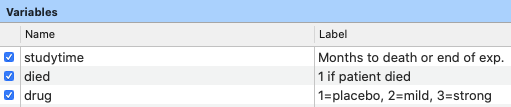
\includegraphics[scale=0.4]{image/label_var}
\end{center}


\begin{verbatim}
. label define drug 1 "placebo" 2 "mild" 3 "strong"
. label values drug drug
\end{verbatim}
\begin{center}
	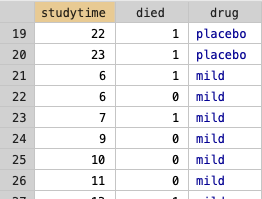
\includegraphics[scale=0.3]{image/label_def}
\end{center}
\end{frame}

%%% 
\subsection{Rename, recode, generate, replace}
\begin{frame}[fragile]{\secname : \subsecname}
\begin{itemize}
\item 	\verb|rename| changes the name of a variable. 
\item[] \verb|. rename died death|
\item   \verb|recode| changes variable values.
\item[] \verb|. recode drug (3=4)|
\item   \verb|generate| creates a new variable.
\item[] \verb|. generate placebo = 1 if drug == 1|
\item   \verb|replace| replaces existing variables (or variable values).
\item[] \verb|. replace placebo = 0 if drug != 1|
\end{itemize}
\end{frame}

%%% 
\subsection{Sort, by, if, in}
\begin{frame}[fragile]{\secname : \subsecname}
s
\end{frame}

%%% 
\subsection{Operators}
\begin{frame}[fragile]{\secname : \subsecname}
\small
\begin{tabulary}{\textwidth}{LLL}
    \toprule
    \textbf{Operator} & \textbf{Purpose} & \textbf{Example} \\
    \midrule
    == & Evaluates if true/false & summarize if sex==1 \\
    $\sim$= or != & Indicates `not equal' & summarize if sex!=0 \\
    $< , <= \newline > , >=$ & Less than (equal to) or greater than (equal to) & summarize if age$<$35 \\
    \& & Indicates `and' & summarize outcome if sex==1 \& age$>=$60 \\
    $ \mid $ & Indicates `or' & gen x=1 if a==1 \& \newline (b==1 $\mid$ c==1) \\
\end{tabulary}
\end{frame}

%%%%
\section{Managing datasets}
\subsection{Merge}
\begin{frame}[fragile]{\secname : \subsecname}
\verb|merge| adds new variables from a second dataset to your existing dataset.
(Make the dataset wider)\\[4mm]
\small
\begin{verbatim}
. use cancer_st, clear // cancer dataset contains only studytime and id
(Patient Survival in Drug Trial)

. merge 1:1 id using cancer_drug12.dta

    Result                           # of obs.
    -----------------------------------------
    not matched                             0
    matched                                34  (_merge==3)
    -----------------------------------------
	
\end{verbatim}

\end{frame}

%%%%
\subsection{Append}
\begin{frame}[fragile]{\secname : \subsecname}
\verb|append| adds new observations to existing variables in your current dataset. \\ (Make the dataset longer) \\[4mm]
\small
\begin{verbatim}
. use cancer_drug12, clear 
(Patient Survival in Drug Trial)

. append using cancer_drug3.dta // append patients using drug 3
\end{verbatim}
\end{frame}

\end{document}